\documentclass[10pt,a4paper,twoside,american]{article}
\usepackage{geometry}
\geometry{verbose,a4paper,tmargin=2cm,bmargin=2cm,lmargin=2cm,rmargin=2cm}
\usepackage[]{float}
\usepackage[table]{xcolor}
\definecolor{shadecolor}{gray}{0.9}
\usepackage{amsmath}
\usepackage{amssymb}
\usepackage{mathtools}
\usepackage{bm}
\usepackage{natbib} 
\usepackage[%%
breaklinks=true,
colorlinks=true,
linkcolor=blue,citecolor=blue,urlcolor=blue,filecolor=blue,
pdffitwindow,
bookmarks=true,
bookmarksopen=true,
bookmarksnumbered=true,
pdftitle={},
pdfauthor={},
pdfsubject={},
pdfkeywords={}
]
{hyperref}
\usepackage{enumitem}

\renewcommand\familydefault{cmss}

%%%%%%%%%%%%%%%%%%%%%%%%%%%%%%%%%%%%%%%%%%%%%%%%%%%%%%%%%%%%%%%%%%%%%%%%%%%%%%%%%%%%
%% macros
\newcommand{\CM}{C_\text{m}}

\newcommand{\drvd}[1]{\textcolor{gray}{#1}} %% font style for derived parameters
\newcommand{\diff}{\ensuremath{\text{d}}}
\newcommand{\dtsim}{\Delta t}
\newcommand{\Epop}{\mathcal{E}} %% set (hence caligraphic) of excitatory neurons
\newcommand{\exc}{\text{E}}     %% label for ``excitatory'
\newcommand{\ext}{\text{X}}   %% label for ``external''
\newcommand{\inh}{\text{I}}     %% label for ``inhibitory''
\newcommand{\Ipop}{\mathcal{I}} %% set (hence caligraphic) of inhibitory neurons
\newcommand{\leak}{\text{L}}              %% label for ``external''
\newcommand{\ms}{\,\text{ms}}
\newcommand{\MOhm}{\,\text{M}\Omega}
\newcommand{\mV}{\,\text{mV}}
\newcommand{\nS}{\,\text{nS}}
\newcommand{\pA}{\,\text{pA}}
\newcommand{\pF}{\,\text{pF}}
\newcommand{\RM}{R_\text{m}}
\newcommand{\sps}{\,\text{spikes/s}}
\newcommand{\Stimulus}{\mathcal{S}} %% set (hence caligraphic) of external spike-train generators
\newcommand{\tauM}{\tau_\text{m}}
\newcommand{\tauR}{\tau_\text{ref}}
\newcommand{\tauS}{\tau_\text{s}}
\newcommand{\note}[1]{\textcolor{red}{[\it #1]}}
\newcommand{\Xpop}{\mathcal{X}} %% set (hence caligraphic) of external spike sources
%%%%%%%%%%%%%%%%%%%%%%%%%%%%%%%%%%%%%%%%%%%%%%%%%%%%%%%%%%%%%%%%%%%%%%%%%%%%%%%%%%%% 
\begin{document}

\title{Model description:\\{\bf TwoPopulationNetworkPlastic}}
\author{}
\date{}
\maketitle
\thispagestyle{empty}
%%%%%%%%%%%%%%%%%%%%%%%%%%%%%%%%%%%%%%%%%%%%%%%%%%%%%%%%%%%%%%%%%%%%%%%%%%%%%%%%%%%%

\def\marg{1ex}
\setlength{\parindent}{0pt}

%%%%%%%%%%%%%%%%%%%%%%%%%%%%%%%%%%%%%%%%%%%%%%%%%%%%%%%%%%%%%%%%%%%%%%%%%%%%%%%%%%%%
%%%%%%%%%%%%%%%%%%%%%%%%%%%%%%%%%%%%%%%%%%%%%%%%%%%%%%%%%%%%%%%%%%%%%%%%%%%%%%%%%%%%
\section{Model description}
\label{sec:model_description}
%%
\renewcommand{\arraystretch}{1.2}
%%
%% model description table
\begin{table}[H]
%%%%%%%%%%%%%%%%%%%
\begin{tabular}{
  |@{\hspace*{\marg}}p{0.2\textwidth-2.\marg}@{\hspace*{\marg}}
  |@{\hspace*{\marg}}p{0.8\textwidth-2.\marg}@{\hspace*{\marg}}
  |}
  \hline 
  \multicolumn{2}{|>{\color{white}\columncolor{black}}c|}{\textbf{Summary}}\\
  \hline 
  \textbf{Populations} & excitatory population $\Epop$, inhibitory population $\Ipop$, external Poissonian spike sources $\Xpop$\\
  \hline 
  \textbf{Connectivity} & sparse random connectivity respecting Dale's principle\\
  \hline 
  \textbf{Neurons} & leaky integrate-and-fire (LIF)
  \\
  \hline 
  \textbf{Synapses} & linear input integration with alpha-shaped postsynaptic currents (PSCs),\\
  & spike-timing dependent plasticity (STDP) for connections between excitatory neurons\\
  \hline 
  \textbf{Input} & stationary, uncorrelated Poissonian spike trains \\
  \hline
  \multicolumn{2}{|c|}{\centering\parbox{0.95\linewidth}{\centering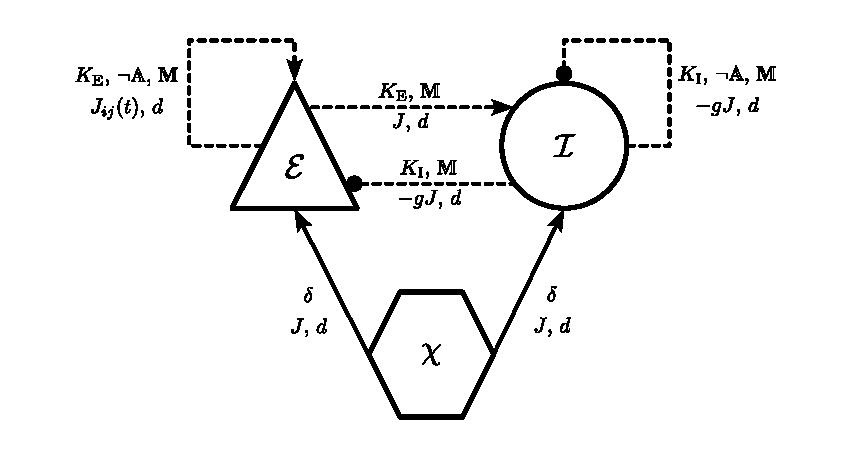
\includegraphics{figures/NetworkSketch_Plastic.pdf}\\[-5ex] \hfill (see \href{https://doi.org/10.1371/journal.pcbi.1010086.g008}{legend})}}\\
  \hline
\end{tabular}
%%%%%%%%%%%%%%%%%%% 
\begin{tabular}{
  |@{\hspace*{\marg}}p{0.2\textwidth-2.\marg}@{\hspace*{\marg}}
  |@{\hspace*{\marg}}p{0.4\textwidth-2.\marg}@{\hspace*{\marg}}
  |@{\hspace*{\marg}}p{0.4\textwidth-2.\marg}@{\hspace*{\marg}}
  |}
  \hline 
  \multicolumn{3}{|>{\color{white}\columncolor{black}}c|}{\textbf{Populations}}\\
  \hline 
  \textbf{Name} & \textbf{Elements} & \textbf{Size}\\
  \hline 
  $\Epop$ & LIF neurons & $N_\exc=\beta{}N$\\
  \hline 
  $\Ipop$ & LIF neurons & $N_\inh=N-N_\exc$\\
  \hline 
  $\Xpop$ & realizations of a Poisson point process & $N$\\
  \hline 
\end{tabular}
%%%%%%%%%%%%%%%%%%%
\caption{Description of the network model (continued on next page).}
\label{tab:model_description}
\end{table}
%%%%%%%%%%%%%%%%%%%%%%%%%%%%%%%%%%%%%%%%%%%%%%%%%%%%%%%%%%%%%%%%%%%%%%%%%%%%%%%%%%%%
%% model description table (continued)
\addtocounter{table}{-1}
\begin{table}[H]
%%%%%%%%%%%%%%%%%%%
%%%%%%%%%%%%%%%%%%% 
\begin{tabular}{
  |@{\hspace*{\marg}}p{0.1\textwidth-2.\marg}@{\hspace*{\marg}}
  |@{\hspace*{\marg}}p{0.1\textwidth-2.\marg}@{\hspace*{\marg}}
  |@{\hspace*{\marg}}p{0.8\textwidth-2.\marg}@{\hspace*{\marg}}
  |}
  \hline 
  \multicolumn{3}{|>{\color{white}\columncolor{black}}c|}{
  \textbf{Connectivity}
  }\\
  \hline 
  \textbf{Source} & \textbf{Target} & \textbf{Pattern}\\
  \hline
  $\Epop$ & $\Epop$ & %
                      \begin{itemize}[align=left,leftmargin=*]
                      \item random, independent; homogeneous in-degree $K_{\exc,i}=K_\exc$ ($\forall{}i\in\Epop$)
                      \item plastic synaptic weights $J_{ij}(t)$ ($\forall{}i\in\Epop,j\in\Epop$)
                      \item homogeneous spike-transmission delays $d_{ij}=d$ ($\forall{}i\in\Epop,j\in\Epop$)
                      \end{itemize}\\
  \hline 
  $\Epop$ & $\Ipop$ & %
                      \begin{itemize}[align=left,leftmargin=*]
                      \item random, independent; homogeneous in-degree $K_{\exc,i}=K_\exc$ ($\forall{}i\in\Ipop$)
                      \item fixed synaptic weights $J_{ij}\in\{0,J\}$ ($\forall{}i\in\Ipop,j\in\Epop$)
                      \item homogeneous spike-transmission delays $d_{ij}=d$ ($\forall{}i\in\Ipop,j\in\Epop$)
                      \end{itemize}\\
  \hline 
  $\Ipop$ & $\Epop\cup\Ipop$ & %
                      \begin{itemize}[align=left,leftmargin=*]
                      \item random, independent; homogeneous in-degree $K_{\inh,i}=K_\inh$ ($\forall{}i\in\Epop\cup\Ipop$)
                      \item fixed synaptic weights $J_{ij}\in\{-gJ,0\}$ ($\forall{}i\in\Epop\cup\Ipop, j\in\Ipop$)                        
                      \item homogeneous spike-transmission delays $d_{ij}=d$ ($\forall{}i\in\Epop\cup\Ipop, j\in\Ipop$)
                      \end{itemize}\\
  \hline 
  $\Xpop$ & $\Epop\cup\Ipop$ & %
                      \begin{itemize}[align=left,leftmargin=*]
                      \item one-to-one
                      \item fixed synaptic weights $J_{ij}=J$ ($\forall{}i\in\Epop\cup\Ipop, j\in\Xpop$)                        
                      \item homogeneous spike-transmission delays $d_{ij}=d$ ($\forall{}i\in\Epop\cup\Ipop, j\in\Xpop$)
                      \end{itemize}\\
  \hline
\multicolumn{3}{|l|}{no self-connections (``autapses''), multiple connections (``multapses'') are permitted}\\
\hline
  \multicolumn{3}{|l|}{all unmentioned connections
  $\Epop\cup\Ipop\to\Xpop$, $\Xpop\to\Xpop$
  are absent}\\
  % \hline
  % all & all & no self-connections (``autapses''), multiple connections (``multapses'') are permitted\\
  \hline
\end{tabular}
%%%%%%%%%%%%%%%%%%%
\begin{tabular}{
  |@{\hspace*{\marg}}p{0.2\textwidth-2.\marg}@{\hspace*{\marg}}
  |@{\hspace*{\marg}}p{0.8\textwidth-2.\marg}@{\hspace*{\marg}}
  |}
  \hline 
  \multicolumn{2}{|>{\color{white}\columncolor{black}}c|}{\textbf{Neuron }}\\
  \hline 
  \textbf{Type} & leaky integrate-and-fire (LIF) dynamics\\
  \hline 
  \textbf{Description} & dynamics of membrane potential $V_{i}(t)$ and spiking activity $s_i(t)$ of neuron $i\in\left\{1,\ldots,N\right\} $:
                         \begin{itemize}
                         \item emission of $k$th ($k=1,2,\ldots$) spike of neuron $i$ at time $t_{i}^{k}$ if
                           \begin{equation*}
                             V_{i}\left(t_{i}^{k}\right)\geq\theta  
                           \end{equation*}
                           with spike threshold $\theta$
                         \item reset and refractoriness:
                           \begin{equation*}
                             \forall{}k,\ \forall t \in \left(t_{k}^{i},\,t_{k}^{i}+\tauR\right]:\quad V_{i}(t)=V_\text{reset}  
                           \end{equation*}
                            with refractory period $\tauR$ and reset potential $V_\text{reset}$
                         \item spike train $\displaystyle s_i(t)=\sum_k \delta(t-t_i^k)$
                         \item subthreshold dynamics of membrane potential $V_{i}(t)$:
                           \begin{equation*}
                             \begin{aligned}
                               &\forall{}k,\ \forall t \notin \left[t_{i}^{k},\,t_{i}^{k}+\tauR\right):\\
                               &\qquad\tauM\frac{\diff{}V_i(t)}{\diff{}t} =
                               \Bigl[E_\text{L}-V_i(t)\Bigr]+\RM I_i(t)
                             \end{aligned}
                           \end{equation*}
                           with membrane time constant $\tauM$, membrane resistance $\RM$, resting potential $E_\text{L}$, and total synaptic input current $I_i(t)$
                         \end{itemize}\\
  \hline 
\end{tabular}
%%%%%%%%%%%%%%%%%%%
\caption{Description of the network model (continued).}
\end{table}
%%%%%%%%%%%%%%%%%%%%%%%%%%%%%%%%%%%%%%%%%%%%%%%%%%%%%%%%%%%%%%%%%%%%%%%%%%%%%%%%%%%%
%% model description table (continued)
\addtocounter{table}{-1}
\begin{table}[H]
%%%%%%%%%%%%%%%%%%% 
%%%%%%%%%%%%%%%%%%% 
\begin{tabular}{
  |@{\hspace*{\marg}}p{0.2\textwidth-2.\marg}@{\hspace*{\marg}}
  |@{\hspace*{\marg}}p{0.8\textwidth-2.\marg}@{\hspace*{\marg}}
  |}
  \hline 
  \multicolumn{2}{|>{\color{white}\columncolor{black}}c|}{
  \textbf{Synapse: transmission}
  }\\
  \hline 
  \textbf{Type} & current-based synapses with alpha-function shaped postsynaptic currents (PSCs)\\
  \hline 
  \textbf{Description} &
                         \begin{itemize}
                         \item total synaptic input current of neuron $i$
                         \begin{equation*}
                           I_i(t)=I_{\exc,i}(t)+I_{\inh,i}(t)+I_{\ext,i}(t)
                         \end{equation*}
                       \item excitatory, inhibitory and external synaptic input currents 
                         \begin{equation*}
                           %I_{P,i}(t)=\sum_{j\in\mathcal{P}}(\text{PSC}_{ij}*s_j)(t)
                           %\quad\text{for}\quad
                           %(P,\mathcal{P})\in\{(\exc,\Epop),(\inh,\Ipop),(\ext,\Xpop)\}
                           %,
                            \begin{aligned}
                              I_{\exc,i}(t)&=\sum_{j\in\Epop}\bigl(\text{PSC}_{ij}*s_j\bigr)(t-d_{ij})\\
                              I_{\inh,i}(t)&=\sum_{j\in\Ipop}\bigl(\text{PSC}_{ij}*s_j\bigr)(t-d_{ij})\\
                              I_{\ext,i}(t)&=\sum_{j\in\Xpop}\bigl(\text{PSC}_{ij}*s_j\bigr)(t-d_{ij})
                            \end{aligned}
                          \end{equation*}
                        with spike trains $s_j(t)$ of local ($j\in\Epop\cup\Ipop$) and external sources ($j\in\Xpop$), spike transmission delays $d_{ij}$, and convolution operator ``$*$'': \mbox{$\displaystyle\bigl(f*g\bigr)(t)=\int_{-\infty}^\infty\text{d}s\,f(s)g(t-s)$})
                       \item alpha-function shaped postsynaptic currents
                         \begin{equation*}
                           \text{PSC}_{ij}(t)=\hat{I}_{ij}e\tauS^{-1}te^{-t/\tauS}\Theta(t)
                         \end{equation*}
                       with synaptic time constant $\tauS$ and 
                       Heaviside function $\Theta(\cdot)$
                       \item[$\curvearrowright$] postsynaptic potential triggered by a single presynaptic spike
                         \begin{equation*}
                           \text{PSP}_{ij}(t)=
                           \hat{I}_{ij}\frac{e}{\tauS\CM}
                           \left(\frac{1}{\tauM}-\frac{1}{\tauS}\right)^{-2}
                           \left(\left(\frac{1}{\tauM}-\frac{1}{\tauS}\right) t e^{-t/\tauS} - e^{-t/\tauS} + e^{-t/\tauM} \right) \Theta(t)                           
                         \end{equation*}
                       \item PSC amplitude (synaptic weight)
                         \begin{equation*}                          
                           \hat{I}_{ij}=\text{max}_t\bigl(\text{PSC}_{ij}(t)\bigr)
                           =\frac{J_{ij}}{J_\text{unit}(\tauM,\tauS,\CM)}
                         \end{equation*}
                         parameterized by PSP amplitude                    
                           $J_{ij}=\text{max}_t\bigl(\text{PSP}_{ij}(t)\bigr)$ 
                       \item[] with unit PSP amplitude (PSP amplitude for $\hat{I}_{ij}=1$):
                         \begin{equation*}
                           J_\text{unit}(\tauM,\tauS,\CM)
                           = \frac{e}{\CM\left(1-\frac{\tauS}{\tauM}\right)}\left( \frac{e^{-t_\text{max}/\tauM} - e^{-t_\text{max}/\tauS}}{\frac{1}{\tauS} - \frac{1}{\tauM}} - t_\text{max}e^{-t_\text{max}/\tauS} \right),
                         \end{equation*}
                       \item[] time to PSP maximum
                         \begin{equation*}
                           t_\text{max} =
                           \frac{1}{\frac{1}{\tauS} - \frac{1}{\tauM}}\left(-W_{-1}\left(\frac{-\tauS e^{-\frac{\tauS}{\tauM}}}{\tauM}\right) - \frac{\tauS}{\tauM}\right),
                         \end{equation*}
                        and  Lambert-W function $\displaystyle W_{-1}(x)$ for $\displaystyle x \ge -1/e$
                         \end{itemize}                        
  \\
  \hline 
\end{tabular}
%%%%%%%%%%%%%%%%%%%
\caption{Description of the network model (continued).}
\end{table}
%%%%%%%%%%%%%%%%%%%%%%%%%%%%%%%%%%%%%%%%%%%%%%%%%%%%%%%%%%%%%%%%%%%%%%%%%%%%%%%%%%%% 
%% model description table (continued)
\addtocounter{table}{-1}
\begin{table}[H]
%%%%%%%%%%%%%%%%%%% 
%%%%%%%%%%%%%%%%%%% 
\begin{tabular}{
  |@{\hspace*{\marg}}p{0.2\textwidth-2.\marg}@{\hspace*{\marg}}
  |@{\hspace*{\marg}}p{0.8\textwidth-2.\marg}@{\hspace*{\marg}}
  |}
  \hline 
  \multicolumn{2}{|>{\color{white}\columncolor{black}}c|}{
  \textbf{Synapse: plasticity}
  }\\
\hline 
\textbf{Type} & spike-timing dependent plasticity (STDP) with power-law weight dependence and all-to-all spike pairing scheme \citep{Morrison07_1437} for connections between excitatory neurons\\
\hline 
  \textbf{Description} &
   dynamics of synaptic weights $J_{ij}(t)$ $\forall{}i\in\Epop, j\in\Epop$:                         
   \begin{equation*}
     \begin{aligned}
       &\forall J_{ij}\ge{}0: \\[1ex]
       &\quad
       \frac{\diff{}J_{ij}}{\diff{}t}=
       \lambda^+f^+(J_{ij})\sum_k x^+_j(t)\delta\Bigl(t-[t_i^k+d_{ij}]\Bigr)
       + \lambda^-f^-(J_{ij})\sum_l x^-_i(t)\delta\Big(t-[t_j^l-d_{ij}]\Bigr)\\[1ex]
       &\forall{}\{t|J_{ij}(t)<0\}: \quad J_{ij}(t)=0  \quad \text{(clipping)}
     \end{aligned}
   \end{equation*}
    with
   \begin{itemize}
    \item pre- and postsynaptic spike times $\{t_j^l|l=1,2,\ldots\}$ and $\{t_i^k|k=1,2,\ldots\}$,
    \item magnitude $\lambda^+=\lambda$ of weight update for causal firing (postsynaptic spike following presynaptic spikes: $t_i^k>t_j^l$),
    \item  magnitude $\lambda^-=-\alpha\lambda$ of weight update for acausal firing (presynaptic spike following postsynaptic spikes: $t_i^k<t_j^l$),
    \item power-law weight dependence $f^+(J_{ij})=J_0(J_{ij}/J_0)^{\mu^+}$ of weight update for causal firing with exponent $\mu^+$ and reference weight $J_0$,
    \item linear weight dependence $f^-(J_{ij})=J_{ij}$ of weight update for acausal firing,
    \item (dendritic) delay $d_{ij}$,
    \item spike trace $x^+_j(t)$ of presynaptic neuron $j$, evolving according to
      \begin{equation*}
        \frac{\diff{}x^+_j}{\diff{}t}=-\frac{x^+_j(t)}{\tau^+}+\sum_l\delta(t-t_j^l)
      \end{equation*}
      with presynaptic spike times $\{t_j^l|l=1,2,\ldots\}$ and time constant $\tau^+$,
    \item spike trace $x^-_i(t)$ of postsynaptic neuron $i$, evolving according to
      \begin{equation*}
        \frac{\diff{}x^-_i}{\diff{}t}=-\frac{x^-_i(t)}{\tau^-}+\sum_k\delta(t-t_i^k)
      \end{equation*}
      with postsynaptic spike times $\{t_i^k|k=1,2,\ldots\}$ and time constant $\tau^-$
    \end{itemize}
    {\footnotesize Note: The above weight update accounts for \emph{all} pairs of pre- and postsynaptic spikes (all-to-all spike pairing scheme). The spike histories and the dependence of the weight update on the time lag of pre- and postsynaptic firing are fully captured by the spike traces $x^+_j(t)$ and $x^-_i(t)$.}
  \\
\hline 
\end{tabular}
%%
%%%%%%%%%%%%%%%%%%%
\caption{Description of the network model (continued).}
\end{table}
%%%%%%%%%%%%%%%%%%%%%%%%%%%%%%%%%%%%%%%%%%%%%%%%%%%%%%%%%%%%%%%%%%%%%%%%%%%%%%%%%%%% 
%% model description table (continued)
\addtocounter{table}{-1}
\begin{table}[H]
%%%%%%%%%%%%%%%%%%%
\begin{tabular}{
  |@{\hspace*{\marg}}p{0.2\textwidth-2.\marg}@{\hspace*{\marg}}
  |@{\hspace*{\marg}}p{0.8\textwidth-2.\marg}@{\hspace*{\marg}}
  |}
  \hline 
  \multicolumn{2}{|>{\color{white}\columncolor{black}}c|}{
  \textbf{Stimulus}
  }\\
\hline 
\textbf{Type} & stationary, uncorrelated Poisson spike trains\\
\hline 
  \textbf{Description} & $N=|\Xpop|$ independent realizations $s_i(t)$ ($i\in\Xpop$) of a Poisson point process with constant rate \mbox{$\nu_\ext(t)=\eta\nu_\theta$}, where
                         \begin{equation*}
                          \label{eq:rheobase_rate_LIF_alpha}
                           \nu_\theta=\frac{\theta-E_\text{L}}{\RM{}\hat{I}_X{}e\tauS}
                         \end{equation*}
                         denotes the rheobase rate, and $\eta$ and $\hat{I}_X=J/J_\text{unit}$ the relative rate and the synaptic weight (PSC amplitude) of external sources\\
  %%
  %%%%%%%%%%%%%%%%%%%%%%%%%%%%%%%%%%%%%%%%%%%%%%%%%%%%%%%%%%%%%%%%%%%%%%%%%%%%%%%%%%%%%%%%%%%%%%%%%%%%%%%
  %% derivation (don't remove this comment):
  %% stationary voltage response to DC current (LIF): V_inf - E_L = R_m I
  %% DC rheobase: V_inf=theta: I_theta = (theta - E_L) / R_m
  %% shot noise mean current (Campbell): mu_theta = nu_X * F
  %% with F = int dt PSC(t) = I*e/tauS int dt t*exp(-t/tauS)*H(t) = I*e * tauS 
  %% shot noise rheobase: mu_theta = I_theta => nu_theta = I_theta/F = (theta - E_L) / (R_m * I*e * tauS)
  %%%%%%%%%%%%%%%%%%%%%%%%%%%%%%%%%%%%%%%%%%%%%%%%%%%%%%%%%%%%%%%%%%%%%%%%%%%%%%%%%%%%%%%%%%%%%%%%%%%%%%%
  %%
\hline 
\end{tabular}
%%%%%%%%%%%%%%%%%%%
\begin{tabular}{
  |@{\hspace*{\marg}}p{0.2\textwidth-2.\marg}@{\hspace*{\marg}}
  |@{\hspace*{\marg}}p{0.8\textwidth-2.\marg}@{\hspace*{\marg}}
  |}
  \hline 
  \multicolumn{2}{|>{\color{white}\columncolor{black}}c|}{
  \textbf{Initial conditions}
  }\\
\hline 
\textbf{Type} & random initial membrane potentials, homogeneous initial synaptic weights and spike traces\\
\hline 
  \textbf{Description} &
  \begin{itemize}
  \item membrane potentials:
    %$V_i(t=0)\sim\mathcal{N}(\mu_{V_0},\sigma_{V_0})$ randomly and independently drawn from a normal distribution with mean $\mu_{V_0}$ and standard deviation $\sigma_{V_0}$ ($\forall{}i$)                          
    $V_i(t=0)\sim\mathcal{U}(V_{0,\text{min}},V_{0,\text{max}})$ randomly and independently drawn from a uniform distribution between $V_{0,\text{min}}$ and $V_{0,\text{max}}$  ($\forall{}i$)                          
  \item synaptic weights: $\hat{I}_{ij}(t=0)=J/J_\text{unit}$ ($\forall{}i\in\Epop, j\in\Epop$)
  \item spike traces: $x_{+,i}(t=0)=x_{-,i}(t=0)=0$ ($\forall{}i\in\Epop$)
  \end{itemize}\\
  \hline 
\end{tabular}
%%%%%%%%%%%%%%%%%%%
\caption{Description of the network model (continued).}
\end{table}
%%%%%%%%%%%%%%%%%%%%%%%%%%%%%%%%%%%%%%%%%%%%%%%%%%%%%%%%%%%%%%%%%%%%%%%%%%%%%%%%%%%%
%%%%%%%%%%%%%%%%%%%%%%%%%%%%%%%%%%%%%%%%%%%%%%%%%%%%%%%%%%%%%%%%%%%%%%%%%%%%%%%%%%%%
\section{Model parameters}
\label{sec:model_parameters}
%%
\renewcommand{\arraystretch}{1.2}
%%
%% parameters table
\def\widthA{0.1}
\def\widthB{0.25}
\def\widthC{0.65}
\begin{table}[H]
  \begin{tabular}{
    |@{\hspace*{\marg}}p{\widthA\textwidth-2.\marg}@{\hspace*{\marg}}
    |@{\hspace*{\marg}}p{\widthB\textwidth-2.\marg}@{\hspace*{\marg}}
    |@{\hspace*{\marg}}p{\widthC\textwidth-2.\marg}@{\hspace*{\marg}}
    |}
    \hline 
    \multicolumn{3}{|>{\columncolor{lightgray}}c|}{\textbf{Network and connectivity}}\\
    \hline 
    \textbf{Name} & \textbf{Value } & \textbf{Description}\\
    \hline 
    $N$ & $12500$ & total number of neurons in local network\\
    \hline 
    $\beta$ & $0.8$ & relative number of excitatory neurons\\
    \hline 
    \drvd{$N_\exc$} & \drvd{$\beta{}N=10000$} & total number of excitatory neurons\\
    \hline 
    \drvd{$N_\inh$} & \drvd{$N-N_\exc=2500$} & total number of inhibitory neurons\\
    \hline 
    $K$ & $1250$ & total number of inputs per neuron (in-degree) from local network\\
    \hline 
    \drvd{$K_\exc$} & \drvd{$\beta{}K=1000$} & number of excitatory inputs per neuron (exc.~in-degree) from local network\\
    \hline 
    \drvd{$K_\inh$} & \drvd{$K-K_\exc=250$} & number of inhibitory inputs per neuron (inh.~in-degree)\\
    \hline 
  %%%%%%%%%%%%%%%%%%%%%%%%%%%%%%%%%%%%%%%%%%%%% 
    \multicolumn{3}{|>{\columncolor{lightgray}}c|}{
    \textbf{Neuron}
    }\\
    \hline 
    \textbf{Name} & \textbf{Value } & \textbf{Description}\\
    \hline 
    $\theta$ & $20\mV$ & spike threshold\\
    \hline 
    $E_\text{L}$ & $0\mV$ & resting potential\\
    \hline 
    $\tauM$ & $20\ms$ & membrane time constant\\
    \hline 
    $\CM$ & $250\pF$ & membrane capacitance\\
    \hline
    \drvd{$\RM$} & \drvd{$\tauM/\CM=80\MOhm$} & membrane resistance\\
    \hline
    $V_\text{reset}$ & $0\mV$ & reset potential\\
    \hline 
    $\tauR$ & $2\ms$ & absolute refractory period\\
    \hline
  %%%%%%%%%%%%%%%%%%%%%%%%%%%%%%%%%%%%%%%%%%%%% 
    \multicolumn{3}{|>{\columncolor{lightgray}}c|}{
    \textbf{Synapse}
    }\\
    \hline 
    \textbf{Name} & \textbf{Value } & \textbf{Description}\\
    %%%%%%%%%%%%%%%%%%%%
    %% transmission
    \hline
    $J$ & $0.5\,\mV$ & (initial) weight (PSP amplitude) of excitatory synapses\\
    \hline
    $g$ & $10$       & relative strength of inhibitory synapses \\
    \hline
    \drvd{$J_\inh$} & \drvd{$-g{}J=-5\,\mV$} & weight (PSP amplitude) of inhibitory synapses\\
    \hline
    \drvd{$J_\text{unit}$} & \drvd{$\approx{}0.01567\,\mV/\pA$} & unit PSP amplitude\\
    \hline
    \drvd{$\hat{I}_\exc(0)$} & \drvd{$J/J_\text{unit}\approx{}31.9\,\pA$} & (initial) weight (PSC amplitude) of excitatory synapses \\
    \hline
    \drvd{$\hat{I}_\inh$} & \drvd{$-g{}J/J_\text{unit}\approx{}-319\,\pA$} & weight (PSC amplitude) of inhibitory synapses \\
    \hline
    \drvd{$\hat{I}_\ext$} & \drvd{$J/J_\text{unit}\approx{}31.9\,\pA$} & weight (PSC amplitude) of external inputs \\
    \hline
    $d$ & $1.5\,\ms$ & spike transmission delay \\
    \hline
    $\tauS$ & $2\,\ms$ & synaptic time constant \\
    \hline
    $\lambda\drvd{=\lambda^+}$ & $20$ & magnitude of weight update for causal firing\\
    \hline
    $\mu^+$ & $0.4$  & weight dependence exponent for causal firing\\
    \hline 
    $J_0$ & $1\,\pA$  & reference weight\\
    \hline 
    $\tau^+$ & $15\,\ms$ & time constant of weight update for causal firing \\
    \hline
    $\alpha$  & $0.1$ & relative magnitude of weight update for acausal firing\\
    \hline
    \drvd{$\lambda^-$} & \drvd{$-\alpha\lambda=-2$} & magnitude of weight update for acausal firing\\
    \hline 
    $\tau^-$ & $30\,\ms$ & time constant of weight update for acausal firing\\
    \hline 
    %%%%%%%%%%%%%%%%%%%%%%%%%%%%%%%%%%%%%%%%%%%%%
    \multicolumn{3}{|>{\columncolor{lightgray}}c|}{
    \textbf{Stimulus}
    }\\
    \hline 
    \textbf{Name} & \textbf{Value } & \textbf{Description}\\
    \hline
    $\eta$ & $1.2$  & relative rate of external Poissonian sources\\
    \hline
    \drvd{$\nu_\theta$} & \drvd{$1442\sps$} & rheobase rate \\ 
    \hline
    \drvd{$\nu_{\ext}$} & \drvd{$\eta\nu_\theta\approx{}1730\sps$} & rate of external Poissonian sources\\
    \hline
  %%%%%%%%%%%%%%%%%%%%%%%%%%%%%%%%%%%%%%%%%%%%% 
    \multicolumn{3}{|>{\columncolor{lightgray}}c|}{
    \textbf{Initial conditions}
    }\\
    \hline 
    \textbf{Name} & \textbf{Value } & \textbf{Description}\\
    \hline
    % $\mu_{V_0}$    & $10\,\mV$ & mean of initial membrane potential distribution\\
    % \hline
    % $\sigma_{V_0}$ & $5\,\mV$  & SD of initial membrane potential distribution\\
    % \hline
    \drvd{$V_{0,\text{min}}$}    & \drvd{$E_\text{L}=0\,\mV$} & minimum initial membrane potential\\
    \hline
    \drvd{$V_{0,\text{max}}$}    & \drvd{$\theta = 20\,\mV$} & maximum initial membrane potential\\
    \hline
  \end{tabular}
  %%%%%%%%%%%%%%%%%%%%%%%%%%%%%%%%%%%%%%%%%%%%% 
  % \begin{tabular}{
  %   |@{\hspace*{\marg}}p{\widthA\textwidth-2.\marg}@{\hspace*{\marg}}
  %   |@{\hspace*{\marg}}p{\widthB\textwidth-2.\marg}@{\hspace*{\marg}}
  %   |@{\hspace*{\marg}}p{\widthC\textwidth-2.\marg}@{\hspace*{\marg}}
  %   |}
  %   \hline 
  %   \multicolumn{3}{|>{\columncolor{lightgray}}c|}{
  %   \textbf{Simulation}
  %   }\\
  %   \hline 
  %   \textbf{Name} & \textbf{Value } & \textbf{Description}\\
  %   \hline 
  %   $T$ & $500\ms$ & total simulation time \\
  %   \hline 
  %   $\dtsim$ & $0.1\ms$ & simulation time resolution \\
  %   \hline
  % \end{tabular}
  %%%%%%%%%%%%%%%%%%%%%%%%%%%%%%%%%%%%%%%%%%%%% 
  \caption{Model parameters. Parameters derived from other parameters are marked in gray.}
  \label{tab:parameters}
\end{table}
%%%%%%%%%%%%%%%%%%%%%%%%%%%%%%%%%%%%%%%%%%%%%%%%%%%%%%%%%%%%%%%%%%%%%%%%%%%%%%%%%%%%
%%%%%%%%%%%%%%%%%%%%%%%%%%%%%%%%%%%%%%%%%%%%%%%%%%%%%%%%%%%%%%%%%%%%%%%%%%%%%%%%%%%% 
%% references
\begin{thebibliography}{}
\bibitem[Morrison et al., 2007]{Morrison07_1437}
  Morrison, A., Aertsen, A., and Diesmann, M.~(2007).
  \newblock Spike-timing-dependent plasticity in balanced random networks.
  \newblock {\em Neural Computation}, 19(6):1437--1467.
\end{thebibliography}

%% NOTE: TwoPopulationNetworkPlastic and the hpc_benchmark https://github.com/nest/nest-simulator/blob/master/pynest/examples/hpc_benchmark.py are exactly identical in their structure and dynamics, except for the shape of the initial membrane potential distribution (which is normal in the hpc_benchmark and uniorm here). Otherwise, the two models differ only in some parameter values, specifically: N, beta, tau_m, tau_ref, tau_s, alpha, lambda, eta, dt



\end{document}
%%% Local Variables:
%%% mode: latex
%%% TeX-master: t
%%% End:
